

In Figure \ref{fig: StokesI_POLI_grid} we present the cleaned images of \SI and polarized intensity, overlaid with the polarization vectors that make up the observed polarization morphologies at \bfourNS, \bfiveNS, \bsix and \bsevenNS. 









% Separate plots
% ----------------------------
% ----------------------------
% \begin{figure*}[h]
%   \centering
% 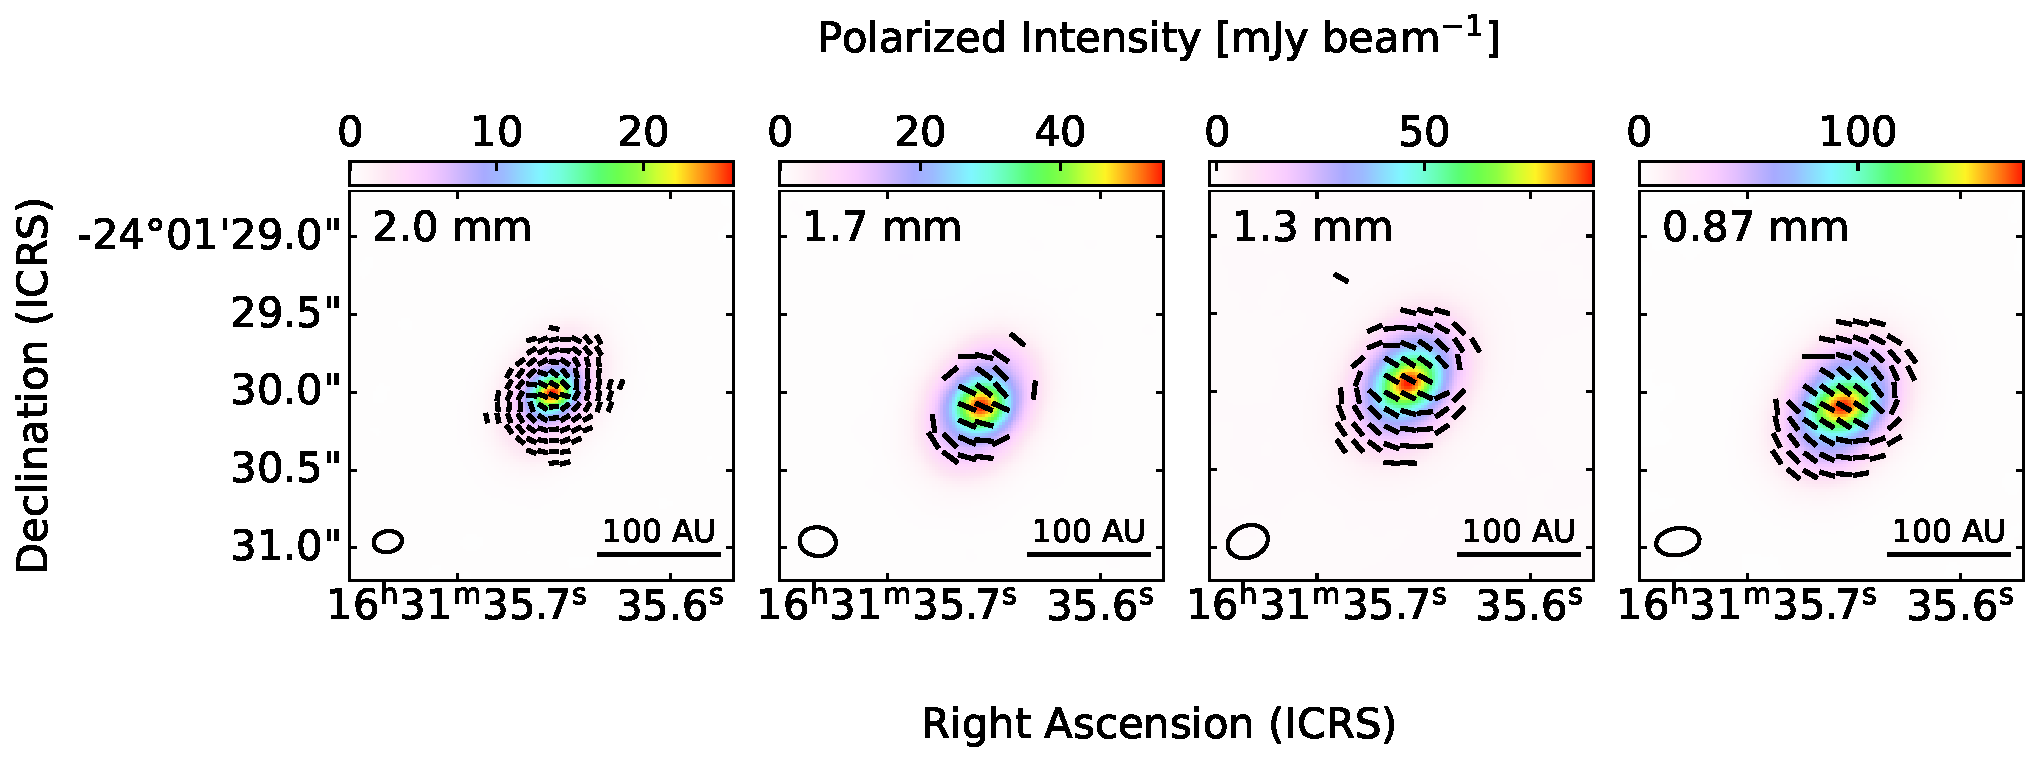
\includegraphics[width=1.1\textwidth]{WRITEUP_AND_IMAGES/IMAGES/WRITEUP/StokesI_POLI/StokesI_grid_robust_minus1.pdf}
%   \caption{Grid of \SI emission for each wavelength of data for IRS 63 with log colour scaling. Polarization vectors are overlaid with black lines of equal length. Vectors are shown only for pixels that satisfy the criteria described in Chapter \ref{sec: methods_vector_criteria}. The beam is shown in the lower left corner, and a reference scale of 100 AU in the top right corner. }
%   \label{fig: StokesI_grid}
% \end{figure*}



% \begin{figure*}[h]
%   \centering
% 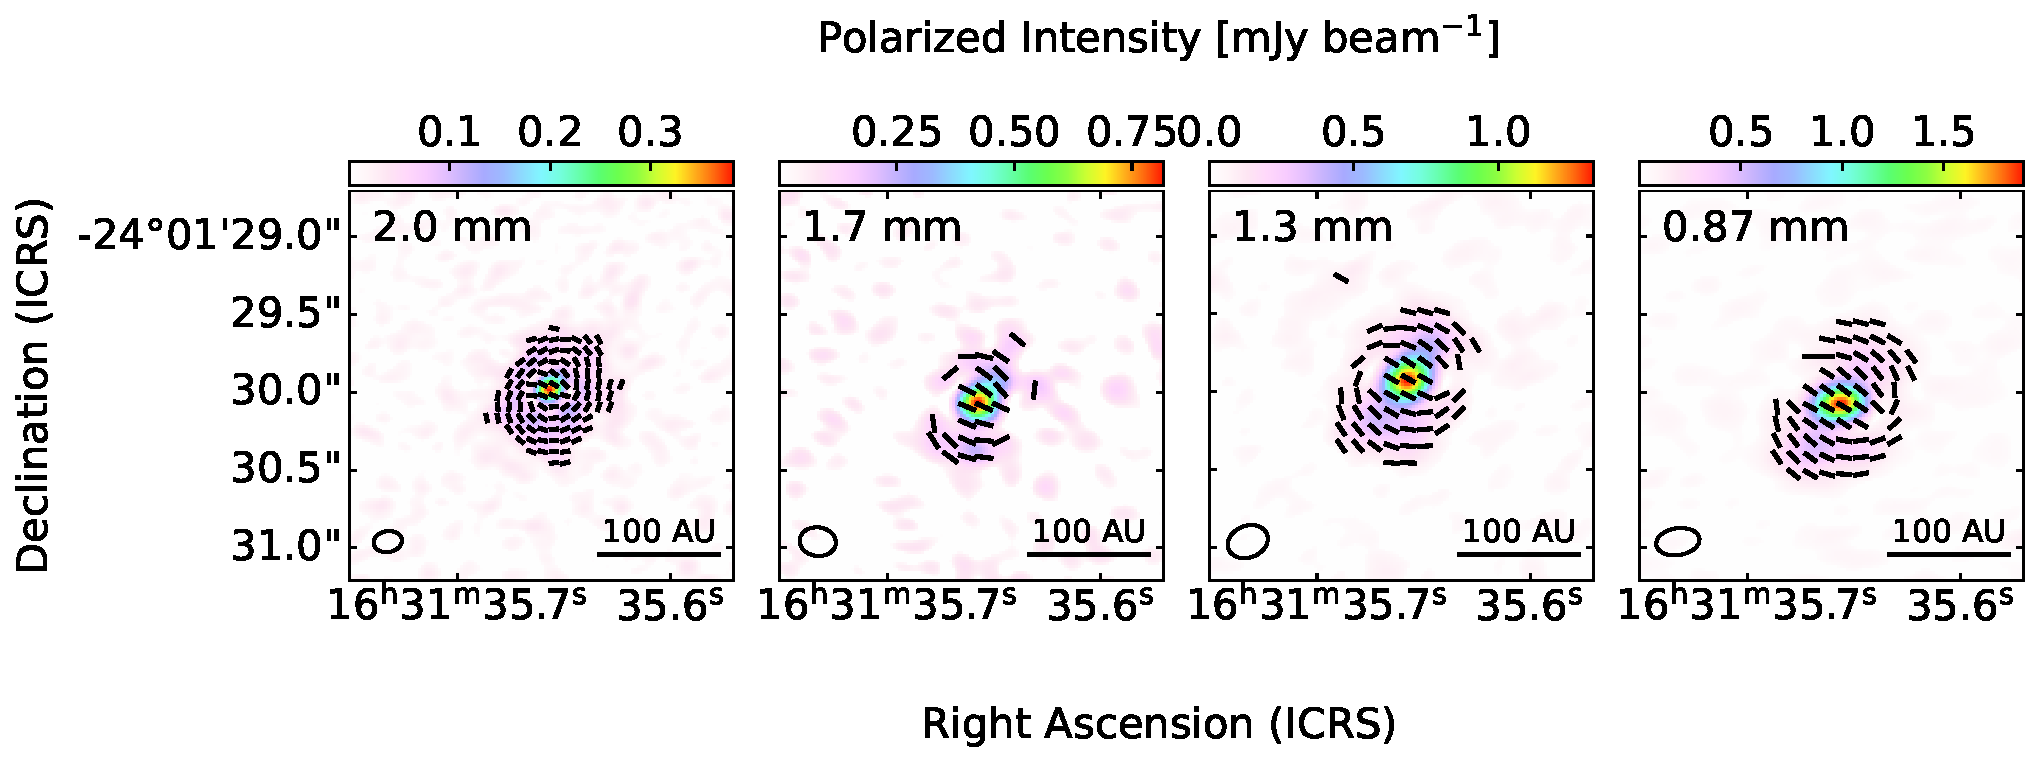
\includegraphics[width=1.1\textwidth]{WRITEUP_AND_IMAGES/IMAGES/WRITEUP/StokesI_POLI/POLI_grid_robust_minus1.pdf}
%   \caption{Same as Figure \ref{fig: StokesI_grid} but for debiased polarized intensity with a linear colour scale}
%   \label{fig: POLI_grid}
% \end{figure*}

% ----------------------------
% ----------------------------



\begin{figure*}[h]
    \centering

    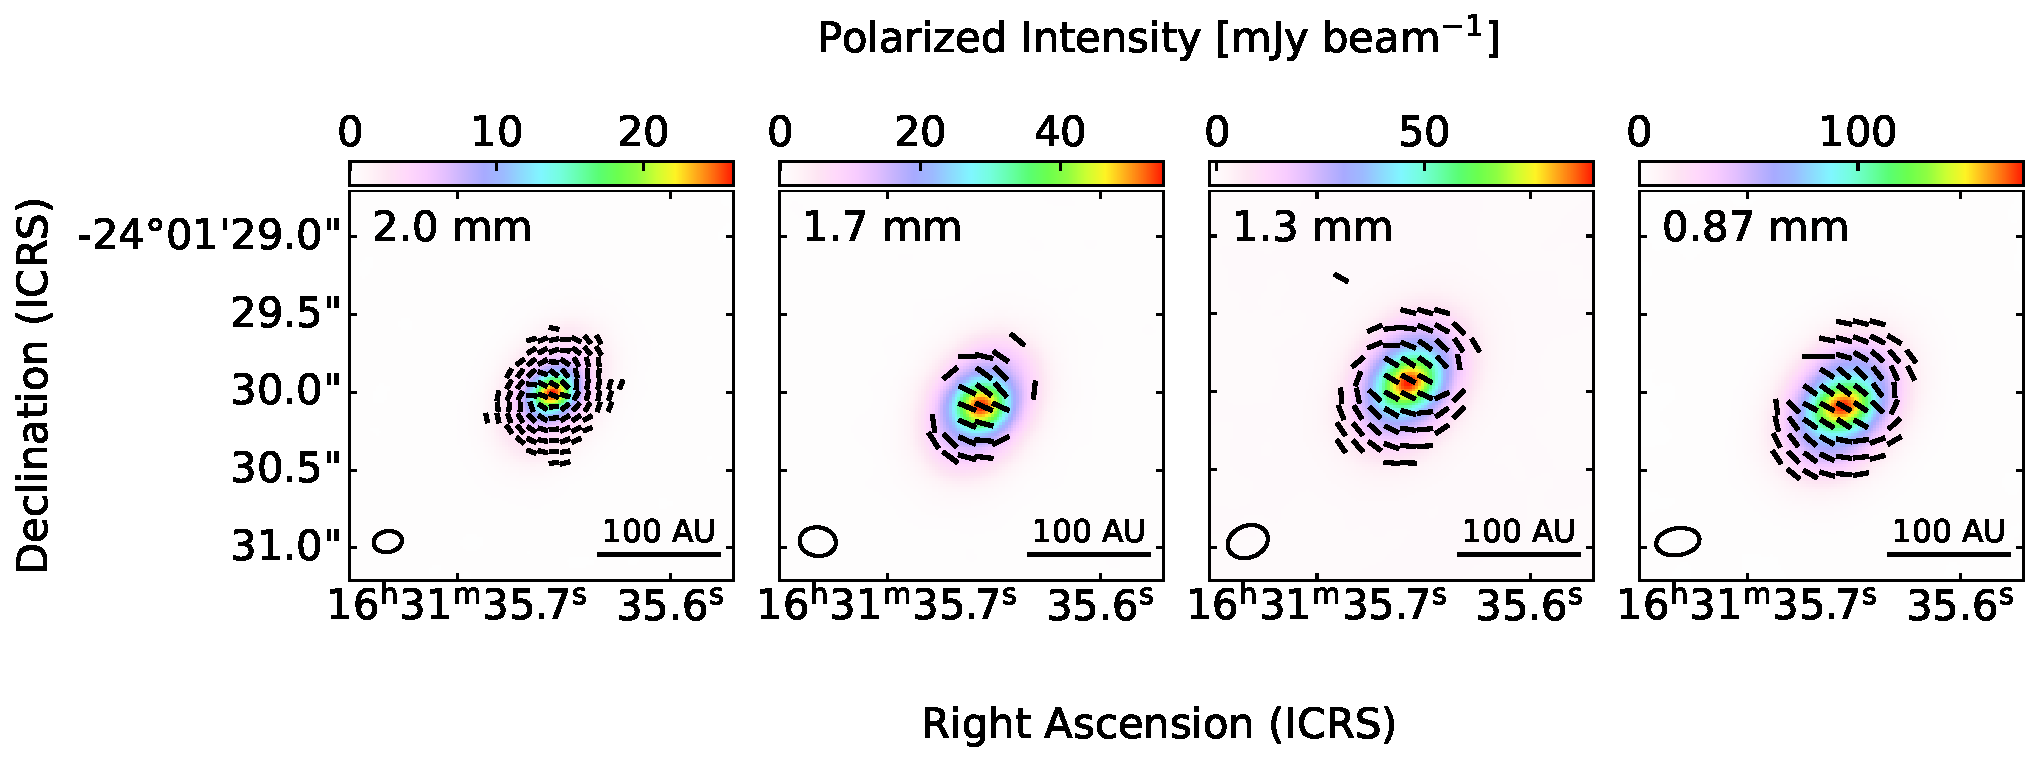
\includegraphics[width=\textwidth]{WRITEUP_AND_IMAGES/IMAGES/WRITEUP/StokesI_POLI/StokesI_grid_robust_minus1.pdf}

    \vspace{0.5cm}

    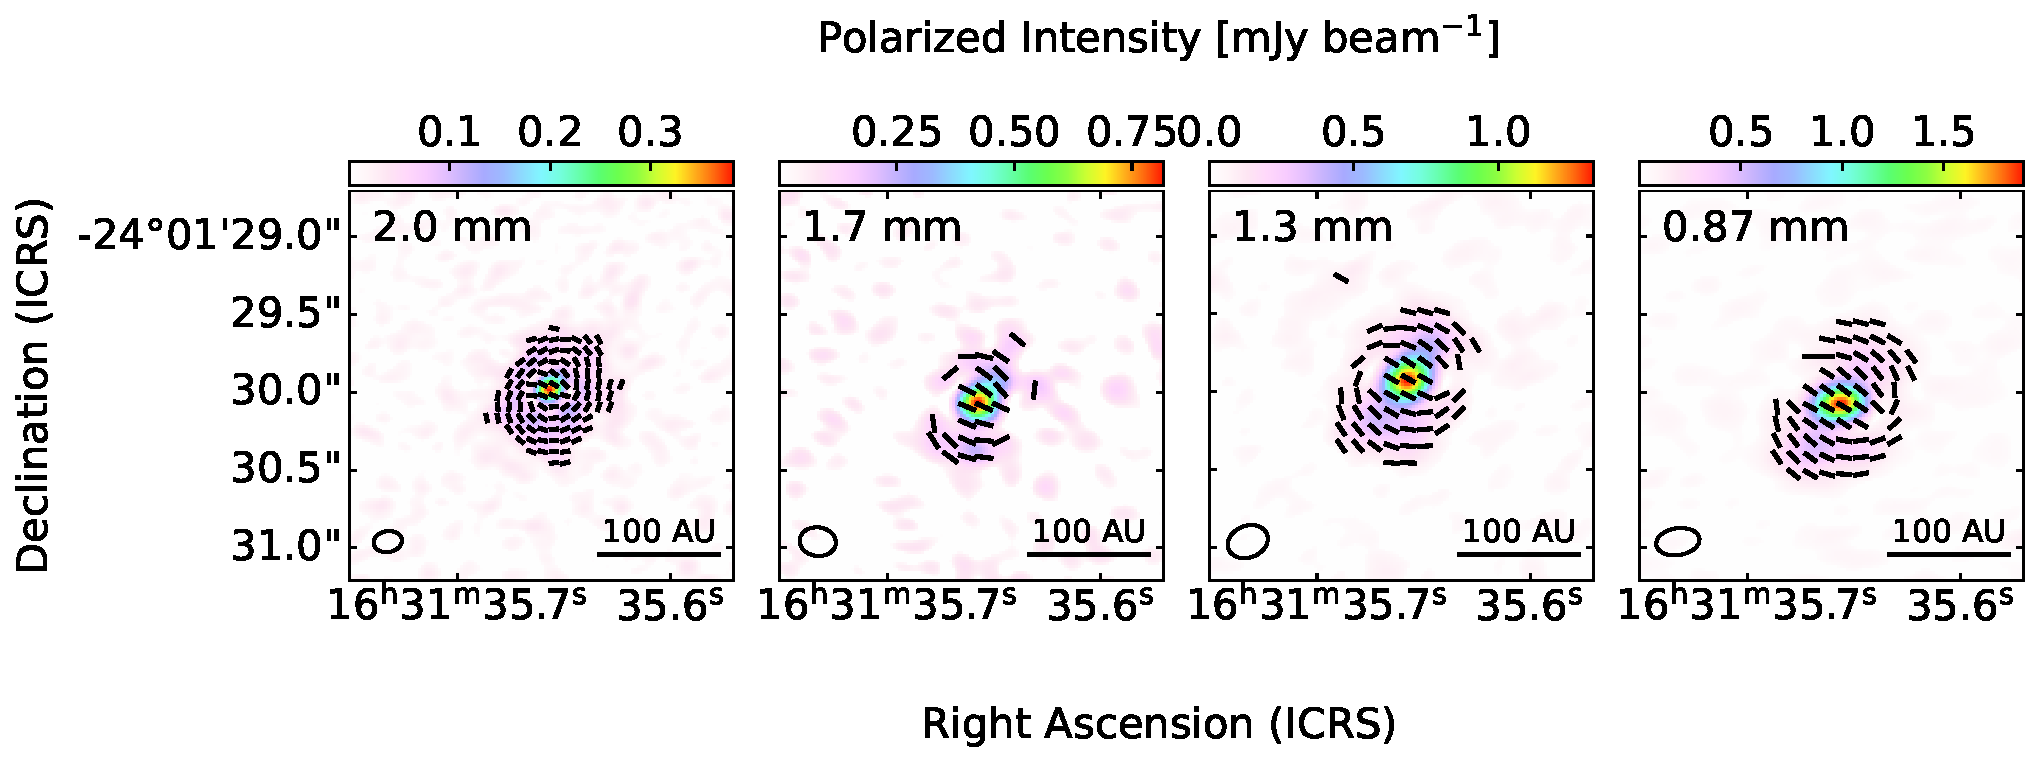
\includegraphics[width=\textwidth]{WRITEUP_AND_IMAGES/IMAGES/WRITEUP/StokesI_POLI/POLI_grid_robust_minus1.pdf}
    \caption{Grid of each wavelength for (Top) \SI emission with log colour scaling and (bottom) debiased polarized intensity with a linear colour scale. Polarization vectors are overlaid with black lines of equal length, showing the change in morphology with wavelength. Vectors are shown only for pixels that satisfy the criteria described in Chapter \ref{sec: methods_vector_criteria}. The beam is shown in the lower left corner, and a reference scale of 100 AU in the top right corner. \question{Caption too descriptive?}}
    \label{fig: StokesI_POLI_grid}
\end{figure*}




% The streamer at \bfive is highlighted in red vectors, and is explained further in Chapter \ref{chap: discussion_streamer}
% ----------------------------










\subsection{Polarization Morphology \note{work on this}}
Using Figure \ref{fig: StokesI_POLI_grid} we examine the transition in polarization morphology, as each wavelength probes a different optical depth. 


At higher wavelengths the polarization morphology resembles the alignment to radiation fields in Figure, \ref{fig: kataoka_polarization_morphologies}, as they are azimuthal (circular) about the centre of the disk.

As wavelength decreases, the polarization morphology resembles the morphology due to self-scattering, as the vectors are uniformly aligned with the minor axis of the disk. The polarization pattern appears to have some azimuthal influence more around the outer part of the disk. The uniform with the minor part of the axis is much more dominant, especially at the sntre of the disk, but spreads further than at higher wavelengths (lower? optical depths).

Similarially, the morphologies also show that even at higher wavelengths there are vectors suggesting self-scattering, but only at the centre of the disk where emission and polarized emission peak. 

 



Additionally, at \bfive and \bsixNS, the two intermediate wavelengths the morphologies are more of a mix, but highlight the transition as radiation to self-scattering is dominant.






 













